\chapter{Revogação de Certificados PGP}

\section{Criação de um Novo Certificado PGP}
Para realizar o experimento de revogação, foi criado um novo certificado PGP específico para teste \cite{gnupgdoc}:

\begin{lstlisting}[language=bash]
gpg --full-generate-key
\end{lstlisting}

\begin{figure}[htb]
    \centering
    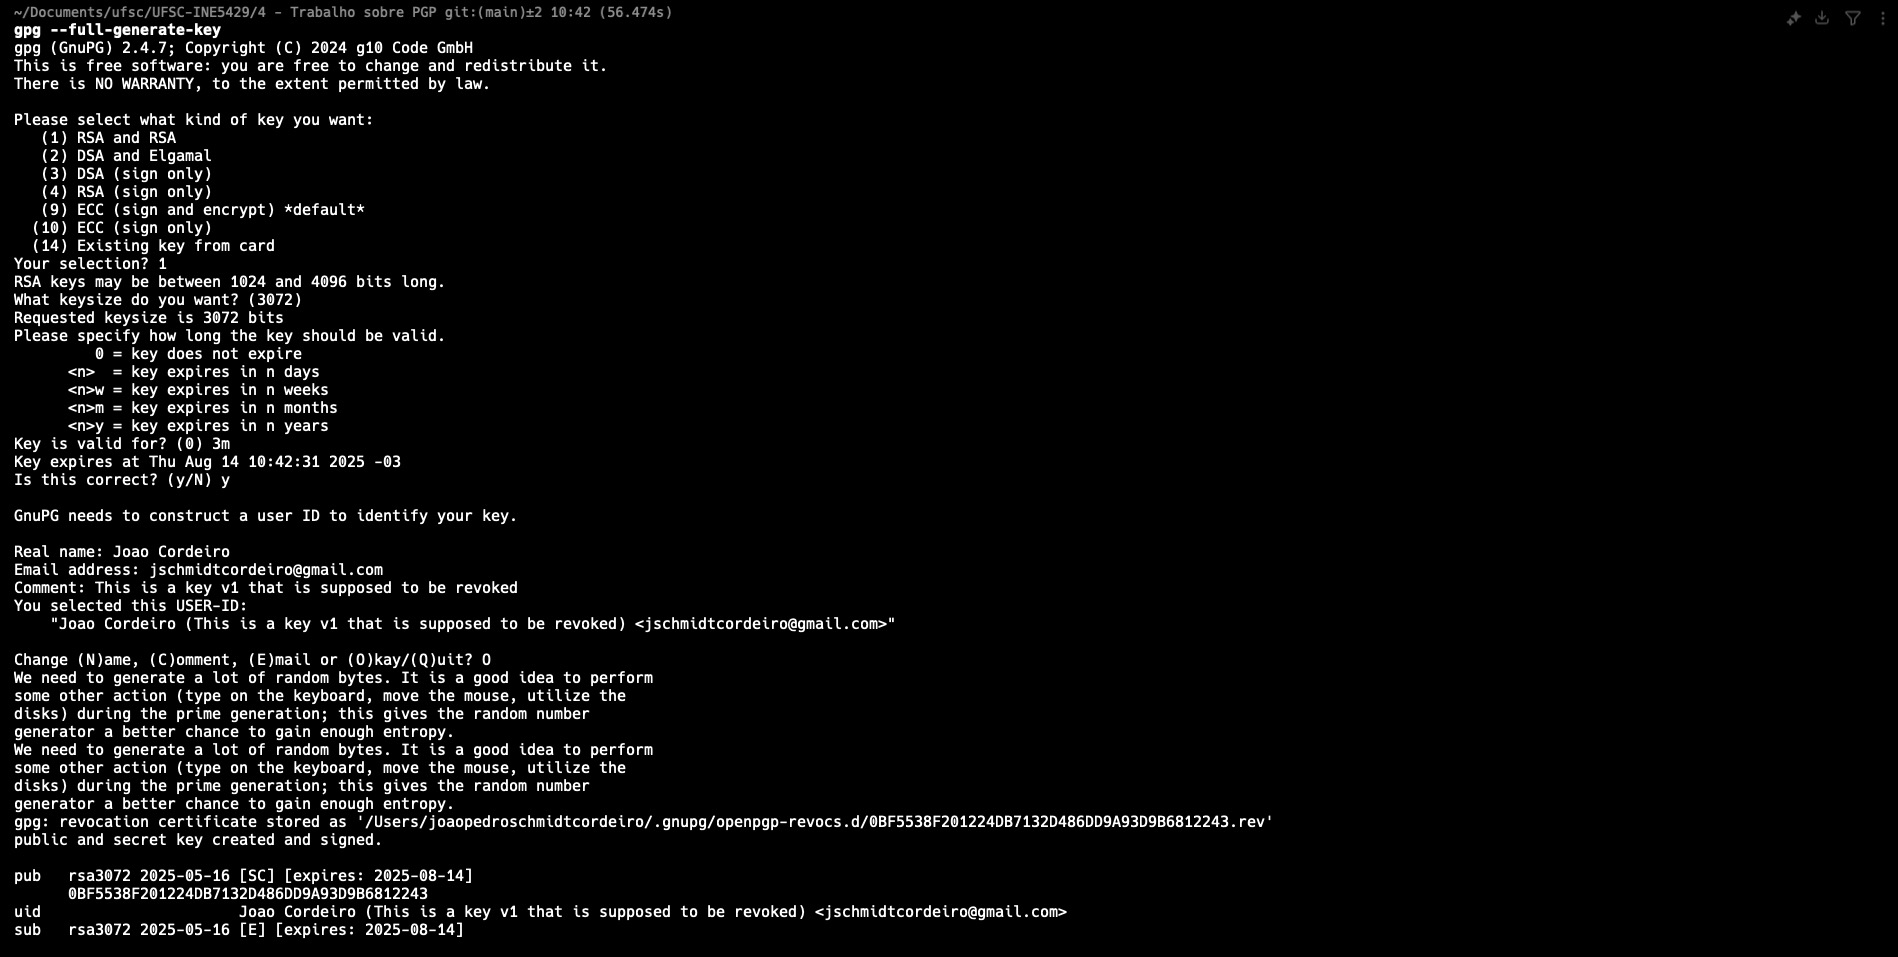
\includegraphics[width=0.8\textwidth]{images/02-criacao_novo_certificado_pgp.jpg}
    \caption{Criação do certificado}
    \label{fig:criacao-certificado}
\end{figure}

Durante o processo interativo:
\begin{enumerate}
    \item Foi selecionado o tipo de chave RSA and RSA (default)
    \item O tamanho da chave foi definido como 3072 bits
    \item O período de validade foi configurado para 90 dias
    \item As seguintes informações foram inseridas:
    \begin{itemize}
        \item Nome: Joao Cordeiro
        \item E-mail: jschmidtcordeiro@gmail.com
        \item Comentário: This is a key v1 that is supposed to be revoked
    \end{itemize}
\end{enumerate}

\section{Publicação no Servidor PGP}
Após criar o certificado, a chave pública foi publicada no servidor de chaves do Ubuntu:

\begin{lstlisting}[language=bash]
# Obtenção do ID da chave gerada
gpg --list-keys jschmidtcordeiro@gmail.com

# Publicação da chave no servidor
gpg --keyserver keyserver.ubuntu.com --send-key 0BF5538F201224DB7132D486DD9A93D9B6812243
\end{lstlisting}

\begin{figure}[htb]
    \centering
    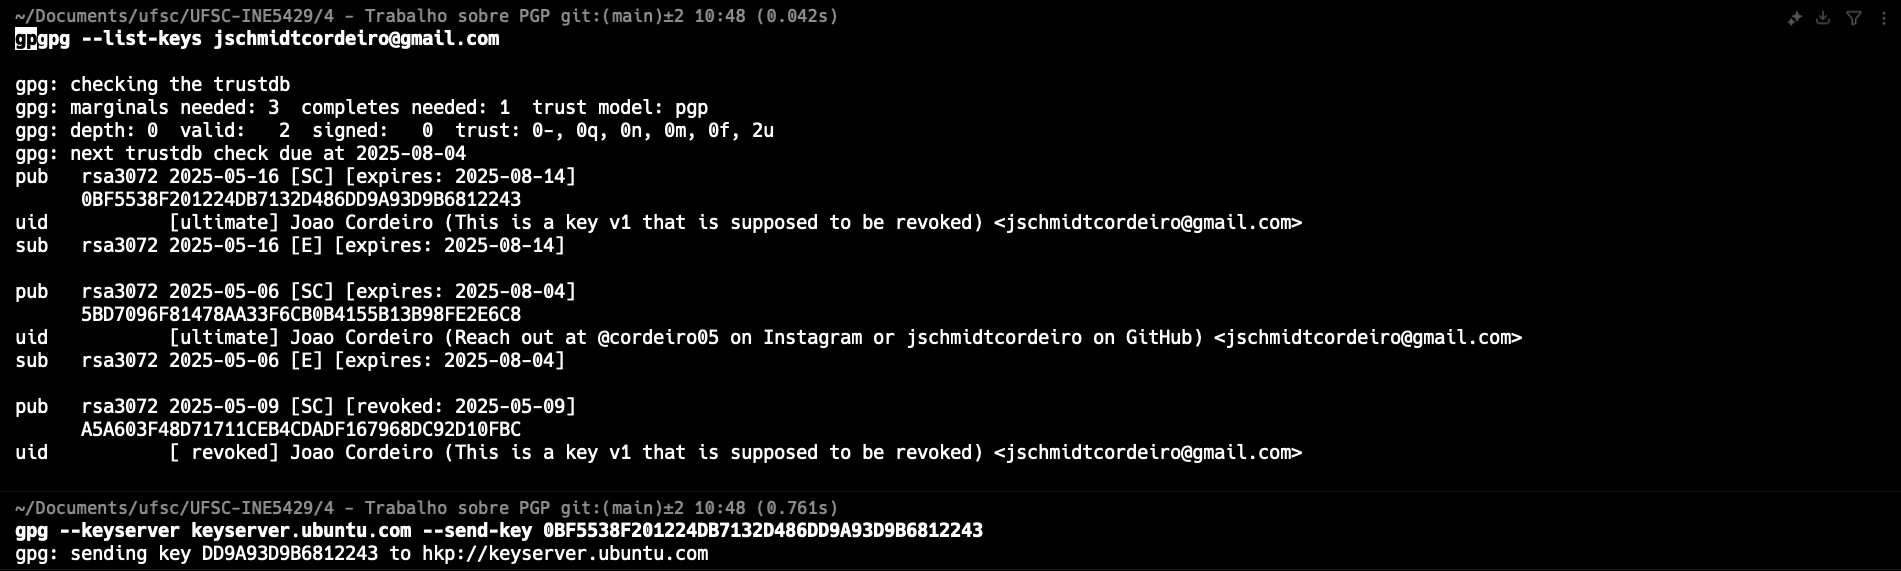
\includegraphics[width=0.8\textwidth]{images/02-publicacao_chave_pgp.jpeg}
    \caption{Publicação da chave}
    \label{fig:publicacao-chave}
\end{figure}

\section{Verificação do Status da Chave}
Para verificar se a chave foi publicada com sucesso:

\begin{lstlisting}[language=bash]
# Atualização do chaveiro local com informações do servidor
gpg --keyserver keyserver.ubuntu.com --refresh-keys

# Verificação do status da chave específica
gpg --keyserver keyserver.ubuntu.com --recv-keys 0BF5538F201224DB7132D486DD9A93D9B6812243
\end{lstlisting}

\begin{figure}[htb]
    \centering
    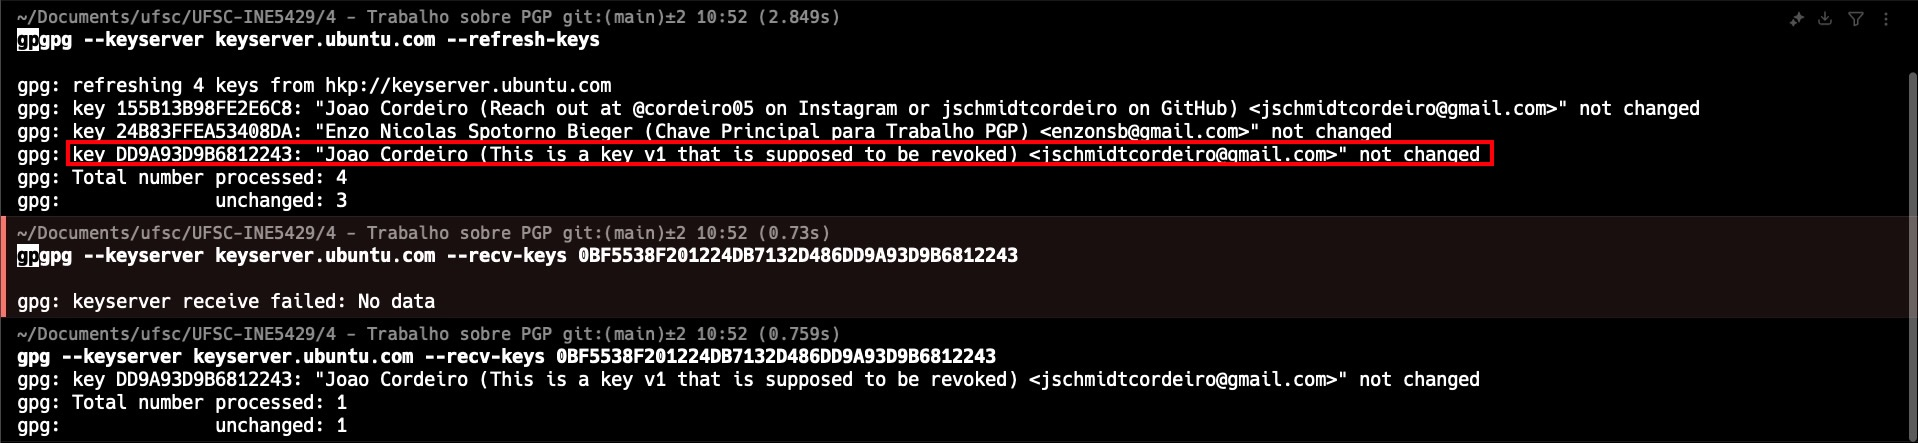
\includegraphics[width=0.8\textwidth]{images/02-verificacao_status_chave.jpeg}
    \caption{Verificação do status da chave}
    \label{fig:verificacao-status}
\end{figure}

\section{Criação do Certificado de Revogação}
Em seguida, foi criado um certificado de revogação para a chave \cite{rfc4880}:

\begin{lstlisting}[language=bash]
# Geração do certificado de revogação
gpg --output revocation_cert.asc --gen-revoke 0BF5538F201224DB7132D486DD9A93D9B6812243
\end{lstlisting}

\begin{figure}[htb]
    \centering
    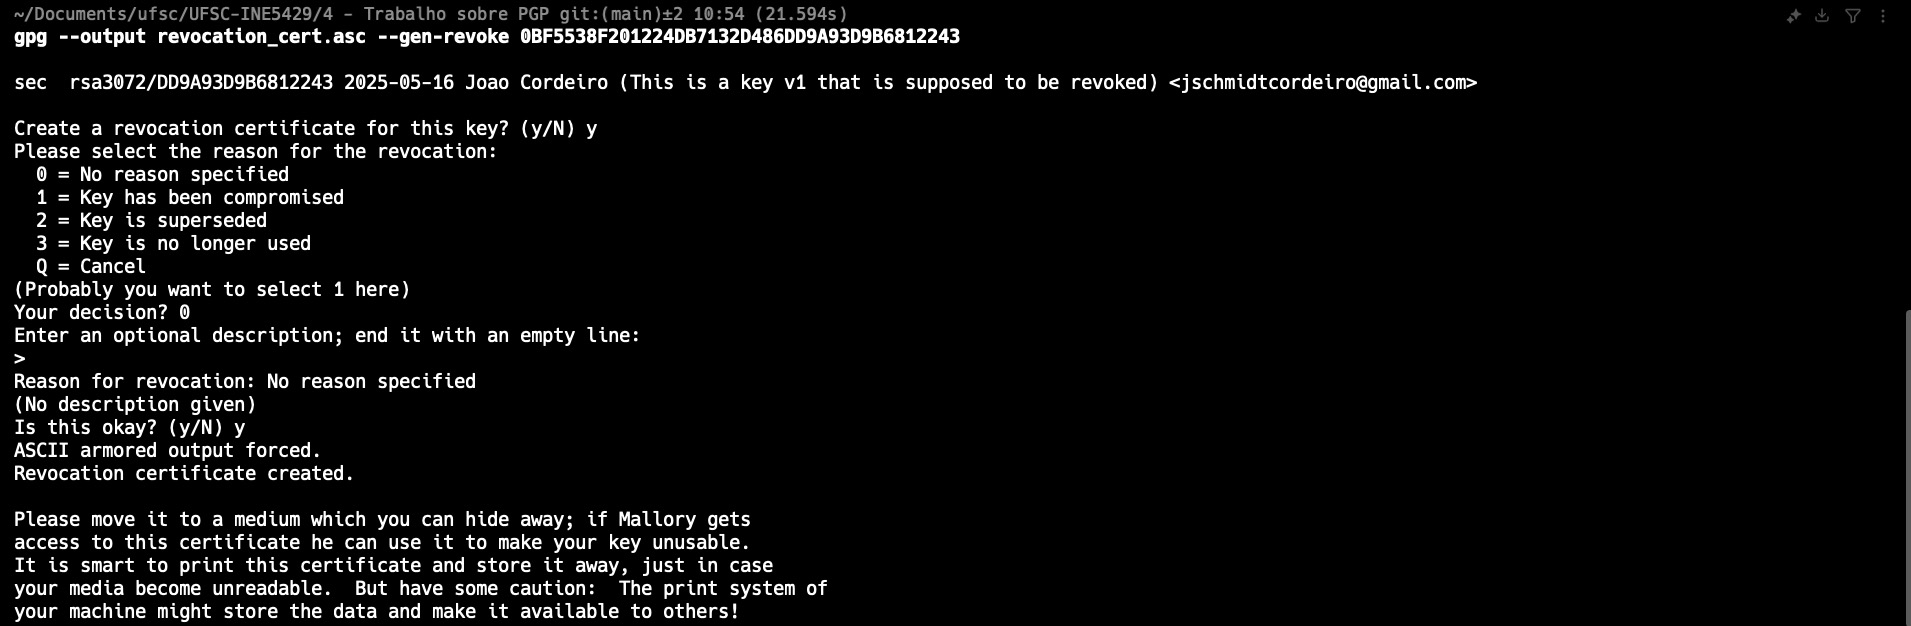
\includegraphics[width=0.8\textwidth]{images/02-criacao_certificado_revogacao.jpg}
    \caption{Criação do certificado de revogação}
    \label{fig:criacao-certificado-revogacao}
\end{figure}

Durante o processo interativo:
\begin{enumerate}
    \item Foi confirmada a criação do certificado de revogação
    \item O motivo da revogação foi selecionado (0 = Sem motivo específico)
    \item Uma descrição vazia foi adicionada
    \item A criação do certificado foi confirmada
\end{enumerate}

\section{Revogação do Certificado}
Com o certificado de revogação gerado, procedeu-se à revogação da chave \cite{rfc4880}:

\begin{lstlisting}[language=bash]
# Importação do certificado de revogação para o chaveiro local
gpg --import revocation_cert.asc

# Envio da chave revogada para o servidor
gpg --keyserver keyserver.ubuntu.com --send-key 0BF5538F201224DB7132D486DD9A93D9B6812243
\end{lstlisting}

\begin{figure}[htb]
    \centering
    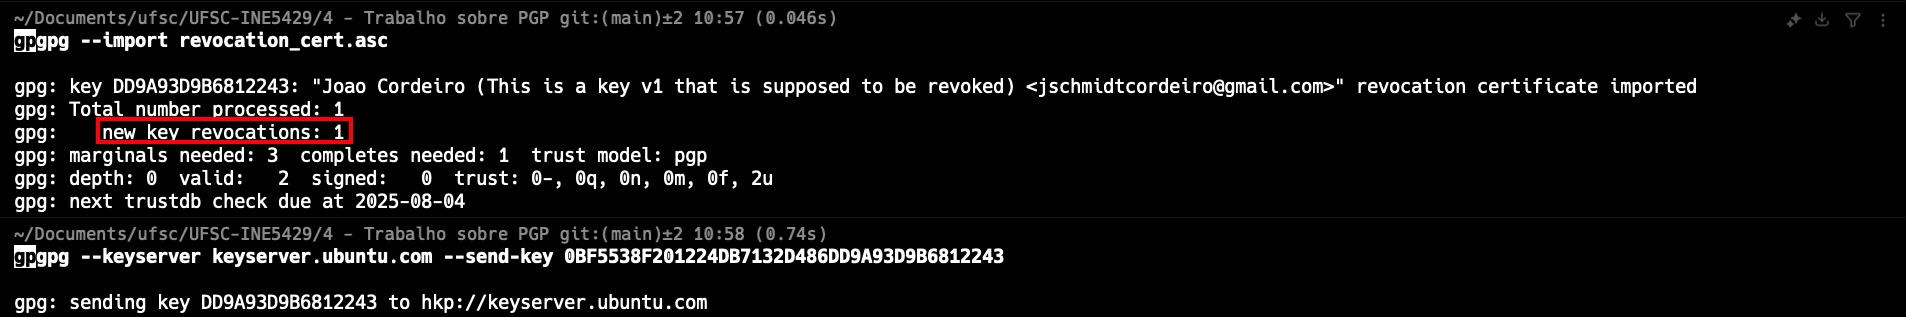
\includegraphics[width=0.8\textwidth]{images/02-revogacao_chave.jpeg}
    \caption{Revogação da chave}
    \label{fig:revogacao-chave}
\end{figure}

\section{Verificação da Revogação}
Para confirmar que a chave foi revogada com sucesso:

\begin{lstlisting}[language=bash]
# Atualização do chaveiro local
gpg --keyserver keyserver.ubuntu.com --refresh-keys

# Verificação do status da chave
gpg --list-keys jschmidtcordeiro@gmail.com
\end{lstlisting}

\begin{figure}[htb]
    \centering
    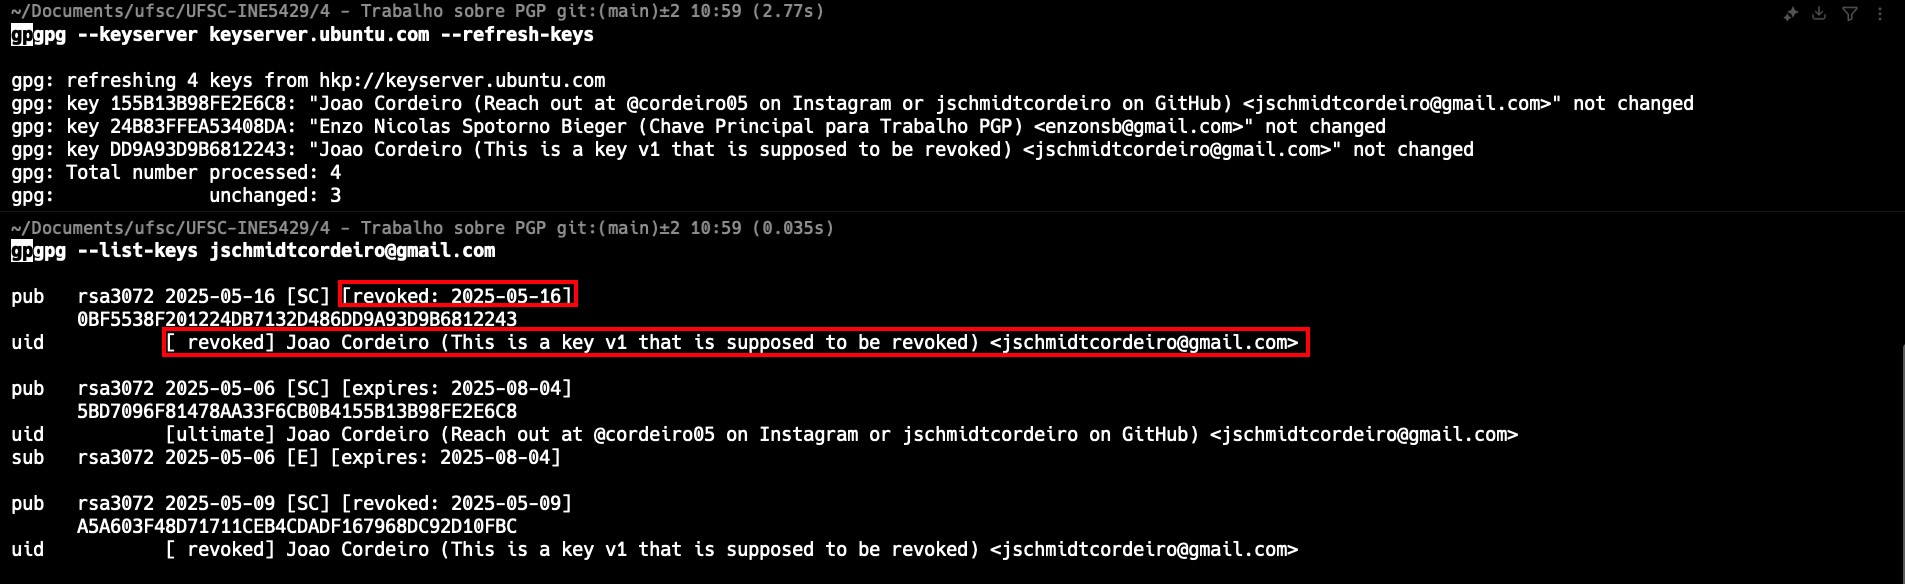
\includegraphics[width=0.8\textwidth]{images/02-verificacao_revogacao_chave.jpeg}
    \caption{Verificação da revogação}
    \label{fig:verificacao-revogacao}
\end{figure}

A saída indica que a chave foi revogada, normalmente com uma marcação como ``rev'' ou ``revoked''.

\section{Resultados do Experimento}

Os resultados de cada comando dos experimentos estão disponíveis nas capturas de tela em suas respectivas seções. As informações principais sobre o certificado revogado são:

\begin{itemize}
    \item \textbf{KeyID do certificado revogado}: 0BF5538F201224DB7132D486DD9A93D9B6812243
    \item \textbf{Data da criação}: 16 de maio de 2025
    \item \textbf{Data da revogação}: 16 de maio de 2025
\end{itemize}